\documentclass[10pt]{article}
\usepackage[utf8]{inputenc}
\usepackage{fullpage}
\usepackage{parskip}
\usepackage{amsmath,amssymb,mathtools}
\usepackage{microtype}
\usepackage{booktabs}
\usepackage{graphicx,subfigure}
\usepackage{algorithm}
\usepackage{url}
\usepackage{makecell}
\usepackage{arydshln}
\usepackage{bm}

\usepackage[most]{tcolorbox}
\newtcolorbox[]{solution}[1][]{%
    breakable,
    enhanced,
    colback=pink,
    title=Solution,
    #1
}

\usepackage{xcolor} %hilight
\newcommand{\hilight}[1]{\colorbox{yellow}{#1}}

\title{10-708 PGM (Spring 2019): Homework 2 \textcolor{red}{v1.1}}
\author{
\begin{tabular}{rl}
Andrew ID: & [your Andrew ID] \\
Name: & [your first and last name] \\
Collaborators: & [Andrew IDs of all collaborators, if any]
\end{tabular}
}
\date{}


\begin{document}

\maketitle

\section{Sequential models for POS tagging [30 pts] (Maruan)}
\label{sec:seq-pos-tagging}

Conditional Random Field (CRF) \cite{lafferty2001crf} is a popular probabilistic model used for structured prediction or modeling conditional probability distributions over structured spaces.
In Homework 1, you have implemented an algorithm for learning parameters of an (unsupervised) Hidden Markov Model (HMM).
In this problem, we will apply a (supervised) HMM and a CRF to part-of-speech (POS) tagging and compare the two models.

In part-of-speech tagging, we are given a sentence and would like to categorize each word (or assign it a tag) to a particular part of speech.
Here is an example:

\begin{verbatim}
    Sentence: The  reaction  in   the  newsroom  was   emotional  .
    POS tags: DET  NOUN      ADP  DET  NOUN      VERB  ADJ        .
\end{verbatim}

In this problem, we will use the universal tagset \cite{petrov2011universal} (which consists of 12 tags), and train and evaluate our algorithms on the Penn Treebank (PTB) corpus.
Download the data from: \url{https://sailinglab.github.io/pgm-spring-2019/assets/assignments/hw2/pos-data.zip}.

The data folder must contain the following files: \texttt{train\_set.npy}, \texttt{test\_set.npy}, \texttt{vocab.txt}, \texttt{tagset.txt}, that correspond to the training sentences, testing sentences, the vocabulary, and the tagset, respectively.

\subsection{POS tagging with HMM [10 pts]}
\label{sec:pos-hmm}

Since assigning POS tags to words outside of context can be very ambiguous (e.g., try to tag ``\emph{the sailor dogs the hatch}''), we need a model that can take into account the whole sequence of words and infer the most likely sequence of corresponding tags.

\begin{enumerate}
    \item \textbf{[1 point]} Denoting the sequence of $T$ words as $\mathbf{x} := (x_1, \dots, x_T)$ and the corresponding sequence of POS tags as $\mathbf{y} := (y_1, \dots, y_T)$, define an HMM for modeling these sequences: (a) specify how you represent observations and latent states, and (b) specify the parameters of your model.

% ---------------------------------
\begin{solution}
\hilight{TODO}
\end{solution}
% ---------------------------------

    \item \textbf{[3 points]} Given a set of tagged training sentences, describe and implement the learning algorithm for your HMM.
    Note that due to sparsity, estimation of emission probabilities requires smoothing (use $\lambda = 0.01$ for smoothing).
    Report the following:
    \begin{itemize}
    \item The obtained state transition matrix $A$ \textcolor{red}{(round or truncate the values in the matrix to a reasonable precision for visualization purposes)}.
    \item The \emph{negative log likelihood} for your HMM on the train and test sets.\footnote{\textcolor{red}{You can report either $-\log P_\theta(\mathbf{x})$ or $-\log P_\theta(\mathbf{x}, \mathbf{y})$, but specify which one you report.}}
    \end{itemize}

% ---------------------------------
\begin{solution}
\hilight{TODO}
\end{solution}
% ---------------------------------

    \item \textbf{[6 pts]} Now having a trained model, we can answer queries such as, \emph{what is the most likely sequence of tags for the given sequence of words?} Mathematically, we answer such queries by solving the following optimization problem:
    \begin{equation}
        \label{eq:hmm-inference}
        \mathbf{y}^\star = \arg\max_{\mathbf{y}} \mathbb{P}_\mathrm{HMM}(\mathbf{y} \mid \mathbf{x})
    \end{equation}
    Describe and implement an efficient algorithm for solving \eqref{eq:hmm-inference} (\emph{hint}: you can use some primitives from the Baum-Welch algorithm that you implemented in HW1).
    Infer the most likely sequences of tags for the test set sentences.
    Report the \textcolor{red}{per-word accuracy} and visualize the confusion matrix between the tags.

% ---------------------------------
\begin{solution}
\hilight{TODO}
\end{solution}
% ---------------------------------

\end{enumerate}


\subsection{POS tagging with a linear-chain CRF [20 pts]}
\label{sec:pos-crf}

POS tagging is a supervised learning problem with sequential inputs and sequential outputs.
Instead of using HMM (a generative model), we could try to directly model the conditional distribution $\mathbb{P}(\mathbf{y} \mid \mathbf{x})$ using the following form:
\begin{equation}
    \label{eq:general-linear-chain-crf}
    \mathbb{P}(\mathbf{y} \mid \mathbf{x}) = \frac{1}{Z(\mathbf{x})} \prod_{t=1}^{T} \Psi_t(y_t, y_{t-1}, \mathbf{x}),
\end{equation}
where $\Psi_t(y_t, y_{t-1}, \mathbf{x})$ is a non-negative potential function that inputs a pair of tags $y_t, y_{t-1}$ and a sequence of words $\mathbf{x}$, and $Z$ is the normalizing constant.

\begin{enumerate}
    \item \textbf{[2 pts]} Show that the conditional distribution, $\mathbb{P}(\mathbf{y} \mid \mathbf{x})$, that results from an HMM is a particular kind of a linear chain CRF (\emph{hint}: write down the complete likelihood for the HMM as a product of exponents).

% ---------------------------------
\begin{solution}
\hilight{TODO}
\end{solution}
% ---------------------------------


    \item \textbf{[2 pts]} Directly modeling $\mathbb{P}(\mathbf{y} \mid \mathbf{x})$ with a CRF allows us to additionally ``featurize'' the model, or in other words, define additional potentials $\Psi_t(y_t, y_{t-1}, \mathbf{x})$ that may depend on non-trivial features extracted from the input sequence.
    Mathematically define a linear chain CRF model that has potentials of the form $\Psi_t(y_t, y_{t-1}, \mathbf{x})$ which are \emph{log-linear functions} of the following features:
    \begin{enumerate}
        \item identity of the given word, $x_t$, \textcolor{red}{and the current tag, $y_t$},
        \item identity for whether $x_t$ is the first word in the sentence, \textcolor{red}{and the current tag, $y_t$},
        \item identity for whether $x_t$ is the last word in the sentence, \textcolor{red}{and the current tag, $y_t$},
        \item identity of the previous word, $x_{t-1}$, \textcolor{red}{and the current tag, $y_t$},
        \item identity of the next word, $x_{t+1}$, \textcolor{red}{and the current tag, $y_t$},
        \item identity for whether $x_t$ contains a capital letter, \textcolor{red}{and the current tag, $y_t$},
        \item \textcolor{red}{identity of the previous tag, $y_t$, and the current tag, $y_t$},
    \end{enumerate}

% ---------------------------------
\begin{solution}
\hilight{TODO}
\end{solution}
% ---------------------------------

    \item \textbf{[2 pts]} Derive an inference algorithm for determining the most likely sequence of POS tags under your CRF model (\emph{hint}: the algorithm should be very similar to the one you designed for HMM in \ref{sec:pos-hmm}).

% ---------------------------------
\begin{solution}
\hilight{TODO}
\end{solution}
% ---------------------------------

    \item \textbf{[2 pts]} Derive a maximum likelihood learning algorithm for your linear chain CRF.

% ---------------------------------
\begin{solution}
\hilight{TODO}
\end{solution}
% ---------------------------------

    \item \textbf{[10 pts]} Implement the learning and inference procedures for CRF that you derived in the previous steps.
    \begin{enumerate}
        \item First, pre-process the training and test data to incorporate the additional features we defined for the potential functions.
        \item Implement the learning and inference algorithms as you described above.
        External libraries that provide complete implementations of CRF models are prohibited (you would get 0/10 credit for this part of the problem).
        However, you can use any external packages for solving optimization problems as building blocks for your algorithms (including PyTorch or TensorFlow).
        \item Finally, train your model on the \texttt{train\_set} and run inference on the \texttt{test\_set}.
        Report the following:
        \begin{enumerate}
            \item The negative log conditional likelihood (i.e., $-\log \mathbb{P}(\mathbf{y} \mid \mathbf{x})$) of your trained CRF model on both training and test sets.
            \item \textcolor{red}{Per-word} accuracy and the confusion matrix for your model predictions on the test set.
        \end{enumerate}
    \end{enumerate}

% ---------------------------------
\begin{solution}
\hilight{TODO}
\end{solution}
% ---------------------------------

    \item \textbf{[2 pts]} As we have seen, HMM and CRF are respectively generative and discriminative approaches to solving the problem of sequence prediction. Discuss advantages/disadvantages of each model. What if we have limited labeled data?

% ---------------------------------
\begin{solution}
\hilight{TODO}
\end{solution}
% ---------------------------------

\end{enumerate}


%% ---------------------------------
% \begin{solution}
% \hilight{TODO}
% \end{solution}
%% ---------------------------------

\newpage

\section{Variational Inference (VI) [40 pts] (Hao)}
\subsection{Warm-up: VI vs. MCMC [10 pts]}
We will compare Variational Inference (VI) with Markov Chain Monte Carlo (MCMC), the two most popular methods for approximate inference. Below are a list of algorithmic properties, or problem cases that you want to choose one of them to solve. For each item, link to either VI or MCMC, and reason briefly with 1-2 sentences.

\begin{enumerate}
    \item \textbf{[1 point]} Inference results are generally closer to target distributions.
% ---------------------------------
\begin{solution}
\hilight{TODO}
\end{solution}
% ---------------------------------
    \item \textbf{[1 point]} Non-parametric.
% ---------------------------------
\begin{solution}
\hilight{TODO}
\end{solution}
% ---------------------------------
    \item \textbf{[1 point]} Amendable to batched computation using GPUs.
% ---------------------------------
\begin{solution}
\hilight{TODO}
\end{solution}
% ---------------------------------
    \item \textbf{[1 point]} Transform inference into optimization problems.
% ---------------------------------
\begin{solution}
\hilight{TODO}
\end{solution}
% ---------------------------------
    \item \textbf{[1 point]} Easier to integrate with back-propagation.
% ---------------------------------
\begin{solution}
\hilight{TODO}
\end{solution}
% ---------------------------------
    \item \textbf{[1 point]} Involves more stochasticity.
% ---------------------------------
\begin{solution}
\hilight{TODO}
\end{solution}
% ---------------------------------
    \item \textbf{[1 point]} Easier to set the termination condition for the computational loop.
% ---------------------------------
\begin{solution}
\hilight{TODO}
\end{solution}
% ---------------------------------
    \item \textbf{[1 point]} Higher variance under limited computational resources.
% ---------------------------------
\begin{solution}
\hilight{TODO}
\end{solution}
% ---------------------------------
    \item \textbf{[1 point]} Problem case: Estimating a topic model with online streaming text data.
% ---------------------------------
\begin{solution}
\hilight{TODO}
\end{solution}
% ---------------------------------
    \item \textbf{[1 point]} Problem case: Estimating a topic model from a very small text corpus.
% ---------------------------------
\begin{solution}
\hilight{TODO}
\end{solution}
% ---------------------------------
    \item \textbf{[Bonus, 1 point]} Problem case: Posterior inference with non-conjugate distributions.
% ---------------------------------
\begin{solution}
\hilight{TODO}
\end{solution}
% ---------------------------------
    \item \textbf{[Bonus, 1 point]} More naturally fit with stick-breaking process.
% ---------------------------------
\begin{solution}
\hilight{TODO}
\end{solution}
% ---------------------------------
\end{enumerate}


\subsection{VI in Practice [30 pts]}
\subsubsection{A Review of the Vanilla LDA [9 pts]}
We have covered the Latent Dirichlet Allocation (LDA)~\cite{blei2003latent}, one of the most successful topic models in class. Given a collection of text documents $\mathcal{D} = \{\bm{w}_d\}_{d=1}^D$,we denote $\bm{w}_d$ as the $d$th document in the corpus, and $\bm{w}_d = \{w_{di}\}_{i=1}^{N_d}$ with $w_{di}$ being the $i$th word in $\bm{w}_d$, and $N_d$ as the number of words in $\bm{w}_d$. LDA assumes each document is generated from a mixture of $K$ topics, with the mixture proportion $\bm{\theta}_d$, where each topic is a multinomial distribution parametrized by $\bm{\beta}_{k}$ over all $V$ words existed in the vocabulary. The generative process of LDA is therefore as follows:

\begin{itemize}
\item For $k = 1 \rightarrow K$:
\begin{itemize}
    \item Draw topic $\bm{\beta}_{k} \sim \mbox{Dirichlet}(\bm{\eta})$.
\end{itemize}
\item For each document $\bm{w}_d \in \mathcal{D}$:
\begin{itemize}
    \item Draw per-document mixture proportion $\bm{\theta}_d \sim \mbox{Dirichlet}(\bm{\alpha})$.
    \item For each word $w_{di} \in \bm{w}_d$:
    \begin{itemize}
        \item Sample a topic indicator $z_{di} \sim \mbox{Multinomial}(\bm{\theta}_d)$
        \item Sample the word $w_{di} \sim \mbox{Multinomial}(\bm{\beta}_{z_{di}})$
    \end{itemize}
\end{itemize}
\end{itemize}
where we have used $\bm{\eta}$ and $\bm{\alpha}$ as the parameters of the two prior Dirichlet distributions for $\bm{\beta}$ and $\bm{\theta}$, respectively. The graphical model diagram of LDA is showed in Figure~\ref{fig:lda}. Answer the following questions about LDA (no need to explain).
%There exist many ways to do posterior inference and parameter estimation for LDA, including variational inference, MCMC, stochastic VI, collapsed

\begin{figure}[!ht]
\centering
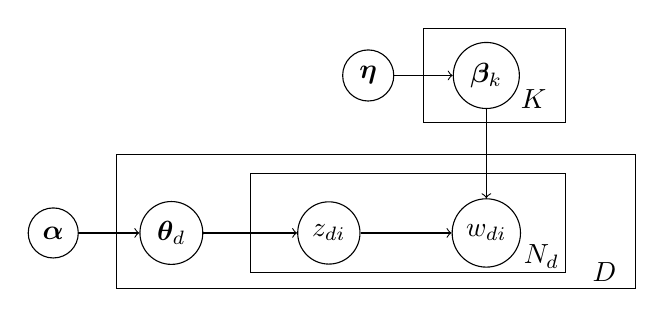
\begin{tikzpicture}
\node (theta) at (0,0) [circle, draw] {$\bm{\theta}_d$};
\node (z) at (2,0) [circle, draw] {$z_{di}$};
\node (w) at (4,0) [circle, draw] {$w_{di}$};
\node (alpha) at (-1.5,0) [circle, draw] {$\bm{\alpha}$};
\node (psis) at (4,2) [circle, draw] {$\bm{\beta}_k$};
\node (b) at (2.5,2) [circle, draw] {$\bm{\eta}$};

\draw[->] (alpha) -- (theta);
\draw[->] (b.east) -- (psis.west);

\draw[->] (theta.east) -- (z.west);
\draw[->] (z.east) -- (w.west);
\draw[->] (psis) -- (w);

\draw (-.7,-.7) rectangle (5.9,1);
\draw (1,-.5) rectangle (5,.75);
\draw (3.2,1.4) rectangle (5,2.6);

\node at (5.5,-.5) {$D$};
\node at (4.7,-.3) {$N_d$};
\node at (4.6,1.7) {$K$};
\end{tikzpicture}
\caption{The graphical model diagram for LDA.}
\label{fig:lda}
\end{figure}

\begin{enumerate}
    \item \textbf{[1 point]} True or False: Solving LDA involves posterior inference with non-conjugate distributions.

% ---------------------------------
\begin{solution}
\hilight{TODO}
\end{solution}
% ---------------------------------

    \item \textbf{[1 point]} True or False: Solving LDA using Variational EM involves non-convex optimization at E-step.

% ---------------------------------
\begin{solution}
\hilight{TODO}
\end{solution}
% ---------------------------------

    \item \textbf{[2 points]} Count the number of \textbf{model parameters} of the LDA using notations defined above.

% ---------------------------------
\begin{solution}
\hilight{TODO}
\end{solution}
% ---------------------------------

    \item \textbf{[2 points]} Write down the computational complexity of mean-field VI for LDA using Big O notation.

% ---------------------------------
\begin{solution}
\hilight{TODO}
\end{solution}
% ---------------------------------

    \item \textbf{[2 points]} Write down the memory complexity of mean-field VI for LDA using Big O notation.

% ---------------------------------
\begin{solution}
\hilight{TODO}
\end{solution}
% ---------------------------------

    \item \textbf{[1 point]} True or False: The vanilla LDA can be used to extract word embeddings.

% ---------------------------------
\begin{solution}
\hilight{TODO}
\end{solution}
% ---------------------------------

\end{enumerate}

\subsubsection{More HMMs [21 pts]}
The vanilla LDA generally assumes each word is independently generated given the topic vectors. In this question, we will try to enhance it by further considering the orders of the words during the document generation process, as we believe in many natural languages, the topic of the word at index $i$ might be dependent on the topic of its previous word (at index $i-1$).

A natural and powerful approach to modeling orders is to (once again) use the Hidden Markov Model (HMM). To incorporate HMM into LDA, we assume a transit matrix $\bm{T}$ among $K$ topics where the entry at the $m$th row and $n$th column of $\bm{T}$, denoted as $\bm{T}_{mn}$, represents the probability of the $m$th topic transiting to the $n$th topic. With $\bm{T}$ introduced, it is convenient for us to model sequential dependencies in the hidden space: instead of sampling each word independently, we let the word $w_{di} (i > 1)$, with probability $p (0 < p <1)$, sampled from the topic $z_{di}$, while with probability $1-p$, transited from the topic $z_{d(i-1)}$, which is the topic indicator of the word $w_{d(i-1)}$. We therefore can alter the generative process as follows:
\begin{itemize}
\item For each document $\bm{w}_d$:
\begin{itemize}
\item Sample $p_d \sim \mbox{Beta}(\gamma)$.
\item Sample $\bm{\theta}_d \sim \mbox{Dirichlet}(\bm{\alpha})$.
\item For the first word (the head of HMM), sample $z_{d1} \sim \mbox{Multinomial}(\bm{\theta}_d), \mbox{ } w_{d1} \sim \mbox{Multimomial}(\beta_{z_{d1}})$.
\item For each word $w_{di}$ $(i > 1)$:
\begin{itemize}
\item Sample $\delta_{di}\sim \mbox{Bernoulli}(p_d)$.
\item If $\delta_{di} = 1$: sample $z_{di}\sim \mbox{Multinomial}(\bm{\theta}_d)$, then $w_{di} \sim \mbox{Multimomial}(\beta_{z_{di}})$.
\item If $\delta_{di} = 0$: sample $z_{di} \sim \mbox{Multinomial}(\bm{T}_{z_{d(i-1)}, :})$, then $w_i \sim \mbox{Multimomial}(\beta_{z_{di}})$.
\end{itemize}
\end{itemize}
\end{itemize}
Where we use $\bm{T}_{m, :}$ to denote the $m$th row of $\bm{T}$.
The posteriors of this model are still intractable, and we will use variational EM to perform posterior inference and estimate model parameters.
\begin{enumerate}
    \item \textbf{[3 points]} Identify (a) the set of observed variables, (b) the set of hidden variables, (c) the set of model parameters to be estimated.

% ---------------------------------
\begin{solution}
\hilight{TODO}
\end{solution}
% ---------------------------------

    \item \textbf{[3 points]} Based on the altered generative process and Figure~\ref{fig:lda}, draw the new graphical model for HMM-enhanced LDA (HMM-LDA).

% ---------------------------------
\begin{solution}
\hilight{TODO}
\end{solution}
% ---------------------------------

    \item \textbf{[2 points]} Write down the joint distribution defined by this generative process.

% ---------------------------------
\begin{solution}
\hilight{TODO}
\end{solution}
% ---------------------------------

    \item \textbf{[3 points]} Define variational distributions over hidden variables using proper distributions and variational parameters.

% ---------------------------------
\begin{solution}
\hilight{TODO}
\end{solution}
% ---------------------------------

    \item \textbf{[2 points]} Derive the ELBO using variational distributions.

% ---------------------------------
\begin{solution}
\hilight{TODO}
\end{solution}
% ---------------------------------

    \item \textbf{[4 points]} Derive the update rules for all variational parameters, which will be used in the E step.

% ---------------------------------
\begin{solution}
\hilight{TODO}
\end{solution}
% ---------------------------------

    \item \textbf{[4 points]} Derive the update rules for all model parameters, which will be applied in the M step.

% ---------------------------------
\begin{solution}
\hilight{TODO}
\end{solution}
% ---------------------------------

    \item \textbf{[Bonus, 6 points]} Implement the derived variational EM algorithm for HMM-LDA using Python ($\ge 3.5$). Train the model on the provided Wikipedia corpus (more details about the dataset can be found in the bundled \texttt{readme.txt}). Set the number of topics $K = 10$.

    \item \textbf{[Bonus, 4 points]} Visualize each of the learned 10 topics by printing its top 10 words with highest probabilities, both in your script and in your write-up.
\end{enumerate}


\textbf{If you choose to do question 8 and 9, please read the implementation notes below carefully before submitting your code}:
    \begin{enumerate}
    \item Only submit a single python script named \texttt{YourAndrewID.py} and a \texttt{requirements.txt} where you put all your needed python requirements. Assuming the dataset file is placed on the same directory path with your script, make sure your script is executable (without bugs) under a clean python ($\ge 3.5$) virtual environment with the following two commands:
    \begin{verbatim}
    pip install -r requirements.txt
    python YourAndrewID.py
    \end{verbatim}
     \item Tune your hyper-parameters properly to make sure the model could converge correctly. Print the values of ELBO after each iteration of E-step and M-step in stdout during the training process. Report the iteration of convergence. Print the value of ELBO after convergence in stdout.
     \item Visualize the learned $K$ topics after convergence in both stdout and the your write-up in a way similar to the upper part of Figure 8 in \cite{blei2003latent}.
    \end{enumerate}

\newpage

\section{Importance Sampling [10 pts] (Paul)}

Given a random distribution $p(x)$ on $x = [x_1,...,x_D]^\top \in \mathbb{R}^D$, suppose we want to perform inference $\mathbb{E}_{p(x)}[f(x)]$ using importance sampling, with $q(x)$ as the proposal distribution. According to importance sampling, we draw $L$ i.i.d. samples $x^{(1)}, ..., x^{(L)}$ from $q(x)$, and we have
\begin{equation}
\mathbb{E}_{p(x)}[f(x)] \approx \frac{1}{\sum_{i=1}^L u_i} \sum_{i=1}^L f(x^{(i)}) u_i
\end{equation}
where the (unnormalized) importance weights $u_i = \frac{p(x^{(i)})}{q(x^{(i)})}$.
%\hilight{XZ:} since variance depends on $ \mathbb{E}_{p(x)} [u_i] $, how about defining $ \mu = \mathbb{E}_{p(x)} [u_i] $ here?

\begin{enumerate}
    \item \textbf{[2 points]} Find the mean and variance of the unnormalized importance weights $\mathbb{E}_{q(x)}[u_i]$ and $\textrm{Var}_{q(x)}[u_i]$. You may leave your answer in terms of $\mathbb{E}_{p(x)}$.

% ---------------------------------
\begin{solution}
    \begin{align*}
        \mathbb{E}_{q(x)}[u_i] &= \int_{x}\frac{p(x)}{q(x)}q(x)dx \\
        &= \int_{x}p(x)dx \\
        &= 1 \\
    \end{align*}

    \begin{align*}
        \textrm{Var}_{q(x)}[u_i] &= \mathbb{E}_{q(x)}[u_i^2] - \left(\mathbb{E}_{q(x)}[u_i]\right)^2\\
        \textrm{Var}_{q(x)}[u_i] &= \mathbb{E}_{q(x)}[u_i^2] - 1 \\
        \textrm{Var}_{q(x)}[u_i] &= \int_{x}\frac{p^2(x)}{q^2(x)}q(x)dx - 1 \\
        \textrm{Var}_{q(x)}[u_i] &= \int_{x}\frac{p^2(x)}{q(x)}dx - 1 \\
        \textrm{Var}_{q(x)}[u_i] &= \int_{x}\frac{p(x)}{q(x)}p(x)dx - 1 \\
        \textrm{Var}_{q(x)}[u_i] &= \mathbb{E}_{p(x)}\left[\frac{p(x)}{q(x)}\right] - 1 \\
    \end{align*}
\end{solution}
% ---------------------------------

    \item \textbf{[3 points]} Prove the following lemma: $\mathbb{E}_{p(x)} \left[\frac{p(x)}{q(x)} \right] \ge 1$ with equality if and only if $p=q$.

% ---------------------------------
\begin{solution}
    By definition, we know that the variance is always $\ge 0$. Hence,
    \begin{align*}
        \textrm{Var}_{q(x)}[u_i] &\ge 0 \\
        \textrm{Var}_{q(x)}[u_i] &= \mathbb{E}_{p(x)}\left[\frac{p(x)}{q(x)}\right] - 1 \\
        \mathbb{E}_{p(x)}\left[\frac{p(x)}{q(x)}\right] - 1 &\ge 0 \\
        \mathbb{E}_{p(x)}\left[\frac{p(x)}{q(x)}\right] &\ge 1 \\
    \end{align*}

    The inequality is clearly equal to $1$ if $p=q$, as the expectation of a constant (here, $1$) is the same constant. \\
    Furthermore, the variance of an R.V is only equal to zero if it is a constant! Hence, for the $\textrm{Var}_{q(x)}[u_i]$ to be equal to zero (i.e. the above equality to hold), $u_i$ should be a constant, which can only happen if $p=q$.
    Hence, \emph{iff} $p=q$, the equality holds.

\end{solution}
% ---------------------------------

    \item \textbf{[4 points]} A measure of the variability of two components in vector $u = [u_1,...,u_L]^\top$ is given by $\mathbb{E}_{q(x)} [(u_i-u_j)^2]$. \color{red}Assume that $p \neq q$ \color{black} and that both $p$ and $q$ can be factorized, i.e. $p(x) = \prod_{i=1}^D p_i(x_i)$, and $q(x) = \prod_{i=1}^D q_i(x_i)$. Show that $\mathbb{E}_{q(x)} [(u_i-u_j)^2]$ has exponential growth with respect to $D$.

% ---------------------------------
\begin{solution}
\begin{align*}
    \mathbb{E}_{q(x)} [(u_i-u_j)^2] &= \mathbb{E}_{q(x)} [u_i^2 + u_j^2 -2u_iu_j] \\
    &= 2\mathbb{E}_{q(x)} [u_i^2] - 2\mathbb{E}_{q(x)}[u_iu_j] \\
    &= 2\mathbb{E}_{q(x)} [u_i^2] - 2 \int_{x_i} \int_{x_j}\frac{p(x_i)}{q(x_i)}\frac{p(x_j)}{q(x_j)} q(x_i) q(x_j) dx_i dx_j \\
    &= 2\mathbb{E}_{q(x)} [u_i^2] - 2 \int_{x_i} \int_{x_j}p(x_i)p(x_j) dx_i dx_j \\
    &= 2\mathbb{E}_{q(x)} [u_i^2] - 2\\
    &= 2\int_{x}\frac{p^2(x)}{q^2(x)} q(x)dx - 2\\
    &= 2\int_{x}\frac{p(x)}{q(x)} p(x)dx - 2\\
    &= 2\mathbb{E}_{p(x)}\left[\frac{p(x)}{q(x)}\right] - 2\\
\end{align*}

Interestingly, this result can be written in terms of the variance that we calculated in the first part. \\
\begin{equation} \label{eq:var_result}
    \mathbb{E}_{q(x)} [(u_i-u_j)^2] = 2 {Var}_{q(x)}[u_i]
\end{equation}
Now, assuming that both $p, q$ can be factorized
\begin{align*}
    \mathbb{E}_{q(x)} [(u_i-u_j)^2] &= 2\mathbb{E}_{p(x)}\left[\frac{p(x)}{q(x)}\right] - 2\\
    \mathbb{E}_{q(x)} [(u_i-u_j)^2] &= 2 \prod_{i=1}^D \mathbb{E}_{p(x_i)}\left[\frac{p(x_i)}{q(x_i)}\right] - 2\\
\end{align*}
From part 2 of the question we know that if $p \neq q$, then  $\mathbb{E}_{p(x_i)} \left[\frac{p(x_i)}{q(x_i)} \right] \ge \alpha$ for some $\alpha \ge 1$. Using this,
\begin{align*}
    \mathbb{E}_{q(x)} [(u_i-u_j)^2] &= 2 \prod_{i=1}^D \mathbb{E}_{p(x_i)}\left[\frac{p(x_i)}{q(x_i)}\right] - 2\\
    \mathbb{E}_{q(x)} [(u_i-u_j)^2] &\ge 2 \alpha^D - 2 \\
\end{align*}
This \emph{blows up} exponentially with the dimension size.
\end{solution}
% ---------------------------------

    \item \textbf{[1 points]} Use the conclusion in (c) to explain why the standard importance sampling does not scale well with dimensionality and would blow up in high-dimensional cases.

% ---------------------------------
\begin{solution}
From the above result, we can see that the difference (in expectation) between the importance scores of two examples from the proposal distribution can blow up with high dimensions. Hence it doesn't scale well with high-dimensional cases.
\end{solution}
% ---------------------------------

\end{enumerate}

\newpage

\section{Markov Chain Monte Carlo [20 pts] (Paul)}

Nowadays, statistical modelling of sport data has become an important part of sports analytics and is often a critical reference for the managers in their decision-making process. In this part, we will work on a real world example in professional sports. Specifically, we are going to use the data from the 2013-2014 Premier League, the top-flight English professional league for men’s football clubs, and build a predictive model on the number of goals scored in a single game by the two opponents. Bayesian hierarchical model is a good candidate for this kind of modeling task. We model each team’s strength (both attacking and defending) as latent variables. Then in each game, the goals scored by the home team is a random variable conditioned on the attacking strength of the home team and the defending strength of the away team. Similarly, the goals scored by the away team is a random variable conditioned on the attack strength of the away team and the defense strength of the home team. Therefore, the distribution of the scoreline of a specific game is dependent on the relative strength between the home team A and the away team B, which also depends on the relative strength between those teams with their other opponents.

\newcolumntype{K}[1]{>{\centering\arraybackslash}p{#1}}

{\fontsize{8}{10}\selectfont
\begin{table*}[h!] %[!htbp]
\caption{2013-2014 Premier League Teams}
\vspace{2mm}
\setlength\tabcolsep{0.7pt}
\begin{tabular}{|c || *{1}{K{3cm}} | *{1}{K{3cm}} | *{1}{K{3cm}} | *{1}{K{3cm}} | *{1}{K{3cm}} |}
\hline
Index & 0 & 1 & 2 & 3 & 4 \\
Team & Arsenal & Aston Villa & Cardiff City & Chelsea & Crystal Palace \\
\hline
\hline
Index & 5 & 6 & 7 & 8 & 9 \\
Team & Everton & Fulham & Hull City & Liverpool & Manchester City \\
\hline
\hline
Index & 10 & 11 & 12 & 13 & 14 \\
Team & Manchester United & Newcastle United & Norwich City & Southampton & Stoke City \\
\hline
\hline
Index & 15 & 16 & 17 & 18 & 19 \\
Team & Sunderland & Swansea City & Tottenham Hotspurs & West Bromwich Albion & West Ham United \\
\hline
\end{tabular}
\label{teams}
\end{table*}
}

Here we consider using the same model as described by Baio and Blangiardo (2010)~\cite{doi:10.1080/02664760802684177}. The Premier League has 20 teams, and we index them as in Table~\ref{teams}. Each team would play 38 matches every season (playing each of the other 19 teams home and away), which totals 380 games in the entire season. For the $g$-th game, assume that the index of home team is $h(g)$ and the index of the away team is $a(g)$.
The observed number of goals $ (y_{g0}, y_{g1}) $ of home and away team is modeled as independent Poisson random variables:
\begin{equation}
y_{gj} | \theta_{gj} \sim \textrm{Poisson}(\theta_{gj}), \quad j = 0,1
\end{equation}
where $\theta = (\theta_{g0},\theta_{g1})$ represents the scoring intensity in the $g$-th game for the team playing at home $(j = 0)$ and away $(j = 1)$, respectively. We put a log-linear model for the $\theta$s:
\begin{equation}
\log \theta_{g0} = home + att_{h(g)} - def_{a(g)}
\end{equation}
\begin{equation}
\log \theta_{g1} = att_{a(g)} - def_{h(g)}
\end{equation}
Note that team strength is broken into attacking and defending strength. And home represents home-team advantage, and in this model is assumed to be constant across teams. The prior on the home is a normal distribution:
\begin{equation}
home \sim \mathcal{N} (0, \tau_0^{-1})
\end{equation}
where we set the precision $\tau_0 = 0.0001$.

The team-specific attacking and defending effects are modeled as:
\begin{equation}
att_t \sim \mathcal{N} (\mu_{att}, \tau_{att}^{-1})
\end{equation}
\begin{equation}
def_t \sim \mathcal{N} (\mu_{def}, \tau_{def}^{-1})
\end{equation}
We use conjugate priors as the hyper-priors on the attack and defense means and precisions:
\begin{equation}
\mu_{att} \sim \mathcal{N} (0, \tau_{1}^{-1})
\end{equation}
\begin{equation}
\mu_{def} \sim \mathcal{N} (0, \tau_{1}^{-1})
\end{equation}
\begin{equation}
\tau_{att} \sim \textrm{Gamma} (\alpha,\beta)
\end{equation}
\begin{equation}
\tau_{def} \sim \textrm{Gamma} (\alpha,\beta)
\end{equation}
where the precision $\tau_1 = 0.0001$, and we set parameters $\alpha = \beta = 0.1$.

This hierarchical Bayesian model can be represented using a directed acyclic graph as shown in Figure~\ref{dag}.

\begin{figure}[ht]
\centering
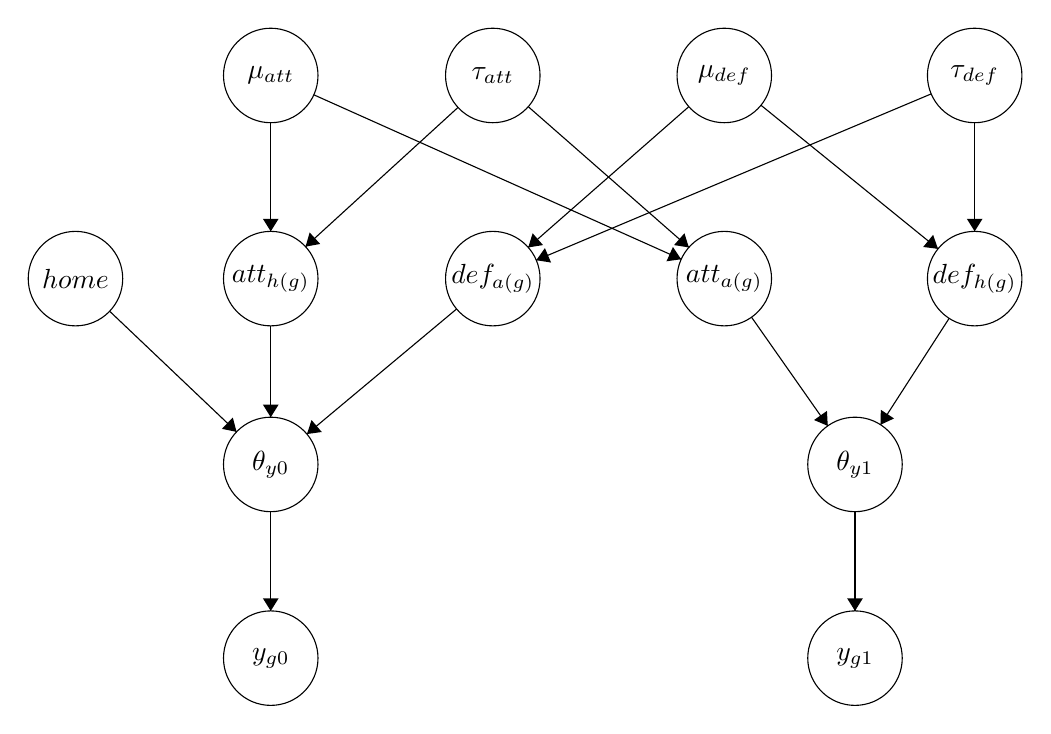
\begin{tikzpicture}[scale=0.2]
\tikzstyle{every node}+=[inner sep=0pt]
\draw [black] (25.1,-42.3) circle (3);
\draw (25.1,-42.3) node {$y_{g0}$};
\draw [black] (62.2,-42.3) circle (3);
\draw (62.2,-42.3) node {$y_{g1}$};
\draw [black] (25.1,-30) circle (3);
\draw (25.1,-30) node {$\theta_{y0}$};
\draw [black] (62.2,-30) circle (3);
\draw (62.2,-30) node {$\theta_{y1}$};
\draw [black] (53.9,-18.2) circle (3);
\draw (53.9,-18.2) node {$att_{a(g)}$};
\draw [black] (69.8,-18.2) circle (3);
\draw (69.8,-18.2) node {$def_{h(g)}$};
\draw [black] (12.7,-18.2) circle (3);
\draw (12.7,-18.2) node {$home$};
\draw [black] (25.1,-18.2) circle (3);
\draw (25.1,-18.2) node {$att_{h(g)}$};
\draw [black] (39.2,-18.2) circle (3);
\draw (39.2,-18.2) node {$def_{a(g)}$};
\draw [black] (39.2,-5.3) circle (3);
\draw (39.2,-5.3) node {$\tau_{att}$};
\draw [black] (25.1,-5.3) circle (3);
\draw (25.1,-5.3) node {$\mu_{att}$};
\draw [black] (53.9,-5.3) circle (3);
\draw (53.9,-5.3) node {$\mu_{def}$};
\draw [black] (69.8,-5.3) circle (3);
\draw (69.8,-5.3) node {$\tau_{def}$};
\draw [black] (25.1,-33) -- (25.1,-39.3);
\fill [black] (25.1,-39.3) -- (25.6,-38.5) -- (24.6,-38.5);
\draw [black] (62.2,-33) -- (62.2,-39.3);
\fill [black] (62.2,-39.3) -- (62.7,-38.5) -- (61.7,-38.5);
\draw [black] (68.18,-20.72) -- (63.82,-27.48);
\fill [black] (63.82,-27.48) -- (64.68,-27.08) -- (63.84,-26.53);
\draw [black] (55.63,-20.65) -- (60.47,-27.55);
\fill [black] (60.47,-27.55) -- (60.42,-26.6) -- (59.6,-27.18);
\draw [black] (69.8,-8.3) -- (69.8,-15.2);
\fill [black] (69.8,-15.2) -- (70.3,-14.4) -- (69.3,-14.4);
\draw [black] (67.04,-6.47) -- (41.96,-17.03);
\fill [black] (41.96,-17.03) -- (42.9,-17.18) -- (42.51,-16.26);
\draw [black] (51.65,-7.28) -- (41.45,-16.22);
\fill [black] (41.45,-16.22) -- (42.39,-16.07) -- (41.73,-15.32);
\draw [black] (56.23,-7.19) -- (67.47,-16.31);
\fill [black] (67.47,-16.31) -- (67.16,-15.42) -- (66.53,-16.19);
\draw [black] (41.45,-7.28) -- (51.65,-16.22);
\fill [black] (51.65,-16.22) -- (51.37,-15.32) -- (50.71,-16.07);
\draw [black] (36.99,-7.33) -- (27.31,-16.17);
\fill [black] (27.31,-16.17) -- (28.24,-16) -- (27.57,-15.27);
\draw [black] (25.1,-8.3) -- (25.1,-15.2);
\fill [black] (25.1,-15.2) -- (25.6,-14.4) -- (24.6,-14.4);
\draw [black] (27.84,-6.53) -- (51.16,-16.97);
\fill [black] (51.16,-16.97) -- (50.64,-16.19) -- (50.23,-17.1);
\draw [black] (14.87,-20.27) -- (22.93,-27.93);
\fill [black] (22.93,-27.93) -- (22.69,-27.02) -- (22,-27.74);
\draw [black] (25.1,-21.2) -- (25.1,-27);
\fill [black] (25.1,-27) -- (25.6,-26.2) -- (24.6,-26.2);
\draw [black] (36.9,-20.13) -- (27.4,-28.07);
\fill [black] (27.4,-28.07) -- (28.34,-27.94) -- (27.69,-27.18);
\end{tikzpicture}
\caption{The DAG representation of the hierarchical Bayesian model. Figure adapted from~\cite{doi:10.1080/02664760802684177}.}
\label{dag}
\end{figure}

The goals of each game are $\mathbf{y} = \{ y_{gj} | g=0,1,...,379, j=0,1 \}$ are the observed variables, and parameters $\boldsymbol{\theta} = \{ home, att_0, def_0, ..., att_{19}, def_{19} \}$ and hyper-parameters $\boldsymbol{\eta} = (\mu_{att}, \mu_{def}, \tau_{att}, \tau_{def})$ are unobserved variables that we need to make inference on. To ensure identifiability, we enforce a corner constraint on the parameters (pinning one team’s parameters to 0,0). Here we use the first team as reference and assign its attacking and defending strength to be 0:
\begin{equation}
att_0 = def_0 = 0
\end{equation}

In this question, we want to estimate the posterior mean of the attacking and defending strength for each team, i.e. $\mathbb{E}_{p(\boldsymbol{\theta},\boldsymbol{\eta}|\mathbf{y})} [att_i]$, $\mathbb{E}_{p(\boldsymbol{\theta},\boldsymbol{\eta}|\mathbf{y})} [def_i]$, and $\mathbb{E}_{p(\boldsymbol{\theta},\boldsymbol{\eta}|\mathbf{y})} [home]$.

\begin{enumerate}
    \item \textbf{[4 points]} Find the joint likelihood $p(\mathbf{y},\boldsymbol{\theta},\boldsymbol{\eta})$.

% ---------------------------------
\begin{solution}
\hilight{TODO}
\end{solution}
% ---------------------------------

    \vspace{10mm}
    \item \textbf{[4 points]} Write down the Metropolis-Hastings algorithm for sampling from posterior $p(\boldsymbol{\theta},\boldsymbol{\eta}|\mathbf{y})$, and derive the acceptance function for a proposal distribution of your choice (e.g. isotropic Gaussian).

% ---------------------------------
\begin{solution}
\hilight{TODO}
\end{solution}
% ---------------------------------

    \item \textbf{[12 points]} Implement the Metropolis-Hastings algorithm to inference the posterior distribution. The data can be found from \url{https://sailinglab.github.io/pgm-spring-2019/assets/assignments/hw2/premier_league_2013_2014.dat}, which contains a $380 \times 4$ matrix. The first column is the number of goals $y_{g0}$ scored by the home team, the second column is the number of goals $y_{g1}$ scored by the away team, the third column is the index for the home team $h(g)$, and the fourth column is the index for the away team $a(g)$.
    \begin{itemize}
        \item Use an isotropic Gaussian proposal distribution $\mathcal{N}(0,\sigma^2I)$ and use \color{red} 0.1 \color{black} as the starting point.
        \item Run the MCMC chain for 5000 steps to burn in and then collect 5000 samples with $t$ steps in between (i.e., run M-H for $5000t$ steps and collect only each $t$-th sample). This is called thinning, which reduces the autocorrelation of the MCMC samples introduced by the Markovian process. The parameter sets are $\sigma = 0.005, 0.05, 0.5$, and $t = 1, 5, 20, 50$.
        \item Plot the trace plot of the burn in phase and the MCMC samples for the latent variable $home$ using proposal distributions with different $\sigma$ and $t$.
        \item Estimate the rejection ratio for each parameter setting, report your results in a table.
        \item Comment on the results. Which parameter setting worked the best for the algorithm?
        \item Use the results from the optimal parameter setting:
        \begin{enumerate}
            \item plot the posterior histogram of variable $home$ from the MCMC samples.
            \item plot the estimated attacking strength $\mathbb{E}_{p(\boldsymbol{\theta},\boldsymbol{\eta}|\mathbf{y})} [att_i]$ against the estimated defending strength $\mathbb{E}_{p(\boldsymbol{\theta},\boldsymbol{\eta}|\mathbf{y})} [def_i]$ for each the team in one scatter plot. Please make sure to identify the team index of each point on your scatter plot using the index to team mapping in Table~\ref{teams}.
        \end{enumerate}
    \end{itemize}

% ---------------------------------
\begin{solution}
\hilight{TODO}
\end{solution}
% ---------------------------------

    \item \textbf{[0 points]} Despite what the data says, conclude that Manchester United is the best team in the Premier League!

\end{enumerate}

\textbf{Note: You are free to use Python or MATLAB for your implementation. You are NOT allowed to use any existing implementations of Metropolis-Hastings in this problem. Please include all the required results (figures + tables) in your writeup PDF submission, as well as submit your code to Gradescope separately.}

\clearpage
\bibliographystyle{unsrt}
\bibliography{references}

\end{document}

\end{solution}
% ---------------------------------

    \item \textbf{[3 points]} Prove the following lemma: $\mathbb{E}_{p(x)} \left[\frac{p(x)}{q(x)} \right] \ge 1$ with equality if and only if $p=q$.

% ---------------------------------
\begin{solution}
\hilight{TODO}
\end{solution}
% ---------------------------------

    \item \textbf{[4 points]} A measure of the variability of two components in vector $u = [u_1,...,u_L]^\top$ is given by $\mathbb{E}_{q(x)} [(u_i-u_j)^2]$. \color{red}Assume that $p \neq q$ \color{black} and that both $p$ and $q$ can be factorized, i.e. $p(x) = \prod_{i=1}^D p_i(x_i)$, and $q(x) = \prod_{i=1}^D q_i(x_i)$. Show that $\mathbb{E}_{q(x)} [(u_i-u_j)^2]$ has exponential growth with respect to $D$.

% ---------------------------------
\begin{solution}
\hilight{TODO}
\end{solution}
% ---------------------------------

    \item \textbf{[1 points]} Use the conclusion in (c) to explain why the standard importance sampling does not scale well with dimensionality and would blow up in high-dimensional cases.

% ---------------------------------
\begin{solution}
\hilight{TODO}
\end{solution}
% ---------------------------------

\end{enumerate}

\newpage

\section{Markov Chain Monte Carlo [20 pts] (Paul)}

Nowadays, statistical modelling of sport data has become an important part of sports analytics and is often a critical reference for the managers in their decision-making process. In this part, we will work on a real world example in professional sports. Specifically, we are going to use the data from the 2013-2014 Premier League, the top-flight English professional league for men’s football clubs, and build a predictive model on the number of goals scored in a single game by the two opponents. Bayesian hierarchical model is a good candidate for this kind of modeling task. We model each team’s strength (both attacking and defending) as latent variables. Then in each game, the goals scored by the home team is a random variable conditioned on the attacking strength of the home team and the defending strength of the away team. Similarly, the goals scored by the away team is a random variable conditioned on the attack strength of the away team and the defense strength of the home team. Therefore, the distribution of the scoreline of a specific game is dependent on the relative strength between the home team A and the away team B, which also depends on the relative strength between those teams with their other opponents.

\newcolumntype{K}[1]{>{\centering\arraybackslash}p{#1}}

{\fontsize{8}{10}\selectfont
\begin{table*}[h!] %[!htbp]
\caption{2013-2014 Premier League Teams}
\vspace{2mm}
\setlength\tabcolsep{0.7pt}
\begin{tabular}{|c || *{1}{K{3cm}} | *{1}{K{3cm}} | *{1}{K{3cm}} | *{1}{K{3cm}} | *{1}{K{3cm}} |}
\hline
Index & 0 & 1 & 2 & 3 & 4 \\
Team & Arsenal & Aston Villa & Cardiff City & Chelsea & Crystal Palace \\
\hline
\hline
Index & 5 & 6 & 7 & 8 & 9 \\
Team & Everton & Fulham & Hull City & Liverpool & Manchester City \\
\hline
\hline
Index & 10 & 11 & 12 & 13 & 14 \\
Team & Manchester United & Newcastle United & Norwich City & Southampton & Stoke City \\
\hline
\hline
Index & 15 & 16 & 17 & 18 & 19 \\
Team & Sunderland & Swansea City & Tottenham Hotspurs & West Bromwich Albion & West Ham United \\
\hline
\end{tabular}
\label{teams}
\end{table*}
}

Here we consider using the same model as described by Baio and Blangiardo (2010)~\cite{doi:10.1080/02664760802684177}. The Premier League has 20 teams, and we index them as in Table~\ref{teams}. Each team would play 38 matches every season (playing each of the other 19 teams home and away), which totals 380 games in the entire season. For the $g$-th game, assume that the index of home team is $h(g)$ and the index of the away team is $a(g)$.
The observed number of goals $ (y_{g0}, y_{g1}) $ of home and away team is modeled as independent Poisson random variables:
\begin{equation}
y_{gj} | \theta_{gj} \sim \textrm{Poisson}(\theta_{gj}), \quad j = 0,1
\end{equation}
where $\theta = (\theta_{g0},\theta_{g1})$ represents the scoring intensity in the $g$-th game for the team playing at home $(j = 0)$ and away $(j = 1)$, respectively. We put a log-linear model for the $\theta$s:
\begin{equation}
\log \theta_{g0} = home + att_{h(g)} - def_{a(g)}
\end{equation}
\begin{equation}
\log \theta_{g1} = att_{a(g)} - def_{h(g)}
\end{equation}
Note that team strength is broken into attacking and defending strength. And home represents home-team advantage, and in this model is assumed to be constant across teams. The prior on the home is a normal distribution:
\begin{equation}
home \sim \mathcal{N} (0, \tau_0^{-1})
\end{equation}
where we set the precision $\tau_0 = 0.0001$.

The team-specific attacking and defending effects are modeled as:
\begin{equation}
att_t \sim \mathcal{N} (\mu_{att}, \tau_{att}^{-1})
\end{equation}
\begin{equation}
def_t \sim \mathcal{N} (\mu_{def}, \tau_{def}^{-1})
\end{equation}
We use conjugate priors as the hyper-priors on the attack and defense means and precisions:
\begin{equation}
\mu_{att} \sim \mathcal{N} (0, \tau_{1}^{-1})
\end{equation}
\begin{equation}
\mu_{def} \sim \mathcal{N} (0, \tau_{1}^{-1})
\end{equation}
\begin{equation}
\tau_{att} \sim \textrm{Gamma} (\alpha,\beta)
\end{equation}
\begin{equation}
\tau_{def} \sim \textrm{Gamma} (\alpha,\beta)
\end{equation}
where the precision $\tau_1 = 0.0001$, and we set parameters $\alpha = \beta = 0.1$.

This hierarchical Bayesian model can be represented using a directed acyclic graph as shown in Figure~\ref{dag}.

\begin{figure}[ht]
\centering
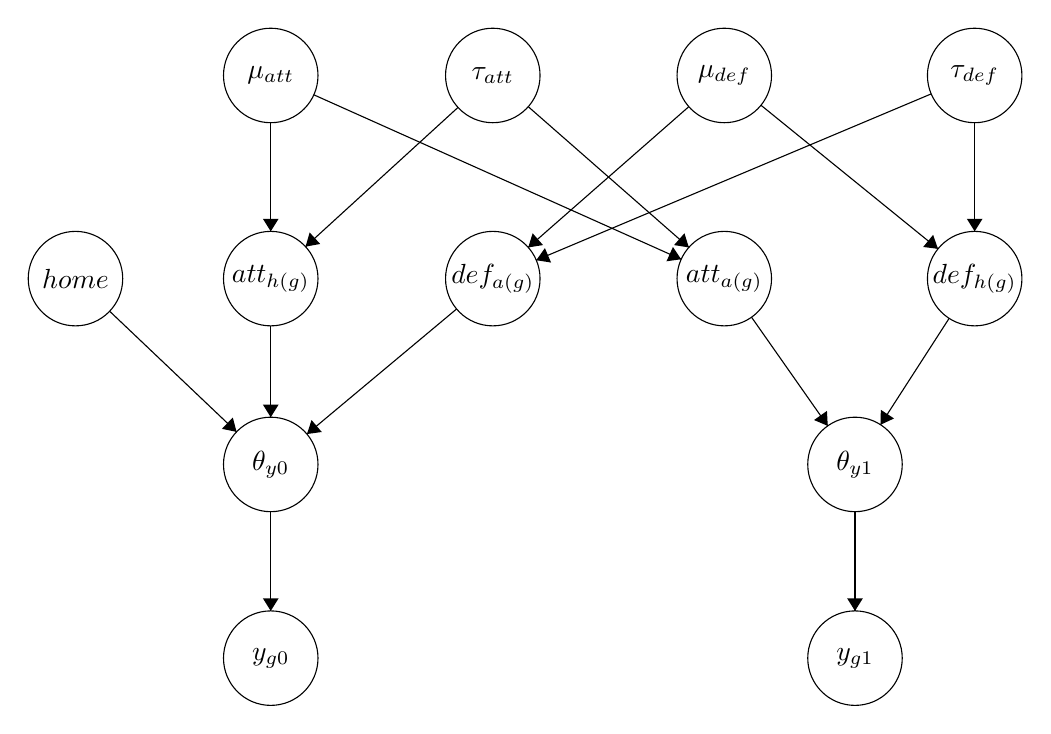
\begin{tikzpicture}[scale=0.2]
\tikzstyle{every node}+=[inner sep=0pt]
\draw [black] (25.1,-42.3) circle (3);
\draw (25.1,-42.3) node {$y_{g0}$};
\draw [black] (62.2,-42.3) circle (3);
\draw (62.2,-42.3) node {$y_{g1}$};
\draw [black] (25.1,-30) circle (3);
\draw (25.1,-30) node {$\theta_{y0}$};
\draw [black] (62.2,-30) circle (3);
\draw (62.2,-30) node {$\theta_{y1}$};
\draw [black] (53.9,-18.2) circle (3);
\draw (53.9,-18.2) node {$att_{a(g)}$};
\draw [black] (69.8,-18.2) circle (3);
\draw (69.8,-18.2) node {$def_{h(g)}$};
\draw [black] (12.7,-18.2) circle (3);
\draw (12.7,-18.2) node {$home$};
\draw [black] (25.1,-18.2) circle (3);
\draw (25.1,-18.2) node {$att_{h(g)}$};
\draw [black] (39.2,-18.2) circle (3);
\draw (39.2,-18.2) node {$def_{a(g)}$};
\draw [black] (39.2,-5.3) circle (3);
\draw (39.2,-5.3) node {$\tau_{att}$};
\draw [black] (25.1,-5.3) circle (3);
\draw (25.1,-5.3) node {$\mu_{att}$};
\draw [black] (53.9,-5.3) circle (3);
\draw (53.9,-5.3) node {$\mu_{def}$};
\draw [black] (69.8,-5.3) circle (3);
\draw (69.8,-5.3) node {$\tau_{def}$};
\draw [black] (25.1,-33) -- (25.1,-39.3);
\fill [black] (25.1,-39.3) -- (25.6,-38.5) -- (24.6,-38.5);
\draw [black] (62.2,-33) -- (62.2,-39.3);
\fill [black] (62.2,-39.3) -- (62.7,-38.5) -- (61.7,-38.5);
\draw [black] (68.18,-20.72) -- (63.82,-27.48);
\fill [black] (63.82,-27.48) -- (64.68,-27.08) -- (63.84,-26.53);
\draw [black] (55.63,-20.65) -- (60.47,-27.55);
\fill [black] (60.47,-27.55) -- (60.42,-26.6) -- (59.6,-27.18);
\draw [black] (69.8,-8.3) -- (69.8,-15.2);
\fill [black] (69.8,-15.2) -- (70.3,-14.4) -- (69.3,-14.4);
\draw [black] (67.04,-6.47) -- (41.96,-17.03);
\fill [black] (41.96,-17.03) -- (42.9,-17.18) -- (42.51,-16.26);
\draw [black] (51.65,-7.28) -- (41.45,-16.22);
\fill [black] (41.45,-16.22) -- (42.39,-16.07) -- (41.73,-15.32);
\draw [black] (56.23,-7.19) -- (67.47,-16.31);
\fill [black] (67.47,-16.31) -- (67.16,-15.42) -- (66.53,-16.19);
\draw [black] (41.45,-7.28) -- (51.65,-16.22);
\fill [black] (51.65,-16.22) -- (51.37,-15.32) -- (50.71,-16.07);
\draw [black] (36.99,-7.33) -- (27.31,-16.17);
\fill [black] (27.31,-16.17) -- (28.24,-16) -- (27.57,-15.27);
\draw [black] (25.1,-8.3) -- (25.1,-15.2);
\fill [black] (25.1,-15.2) -- (25.6,-14.4) -- (24.6,-14.4);
\draw [black] (27.84,-6.53) -- (51.16,-16.97);
\fill [black] (51.16,-16.97) -- (50.64,-16.19) -- (50.23,-17.1);
\draw [black] (14.87,-20.27) -- (22.93,-27.93);
\fill [black] (22.93,-27.93) -- (22.69,-27.02) -- (22,-27.74);
\draw [black] (25.1,-21.2) -- (25.1,-27);
\fill [black] (25.1,-27) -- (25.6,-26.2) -- (24.6,-26.2);
\draw [black] (36.9,-20.13) -- (27.4,-28.07);
\fill [black] (27.4,-28.07) -- (28.34,-27.94) -- (27.69,-27.18);
\end{tikzpicture}
\caption{The DAG representation of the hierarchical Bayesian model. Figure adapted from~\cite{doi:10.1080/02664760802684177}.}
\label{dag}
\end{figure}

The goals of each game are $\mathbf{y} = \{ y_{gj} | g=0,1,...,379, j=0,1 \}$ are the observed variables, and parameters $\boldsymbol{\theta} = \{ home, att_0, def_0, ..., att_{19}, def_{19} \}$ and hyper-parameters $\boldsymbol{\eta} = (\mu_{att}, \mu_{def}, \tau_{att}, \tau_{def})$ are unobserved variables that we need to make inference on. To ensure identifiability, we enforce a corner constraint on the parameters (pinning one team’s parameters to 0,0). Here we use the first team as reference and assign its attacking and defending strength to be 0:
\begin{equation}
att_0 = def_0 = 0
\end{equation}

In this question, we want to estimate the posterior mean of the attacking and defending strength for each team, i.e. $\mathbb{E}_{p(\boldsymbol{\theta},\boldsymbol{\eta}|\mathbf{y})} [att_i]$, $\mathbb{E}_{p(\boldsymbol{\theta},\boldsymbol{\eta}|\mathbf{y})} [def_i]$, and $\mathbb{E}_{p(\boldsymbol{\theta},\boldsymbol{\eta}|\mathbf{y})} [home]$.

\begin{enumerate}
    \item \textbf{[4 points]} Find the joint likelihood $p(\mathbf{y},\boldsymbol{\theta},\boldsymbol{\eta})$.

% ---------------------------------
\begin{solution}
\hilight{TODO}
\end{solution}
% ---------------------------------

    \vspace{10mm}
    \item \textbf{[4 points]} Write down the Metropolis-Hastings algorithm for sampling from posterior $p(\boldsymbol{\theta},\boldsymbol{\eta}|\mathbf{y})$, and derive the acceptance function for a proposal distribution of your choice (e.g. isotropic Gaussian).

% ---------------------------------
\begin{solution}
\hilight{TODO}
\end{solution}
% ---------------------------------

    \item \textbf{[12 points]} Implement the Metropolis-Hastings algorithm to inference the posterior distribution. The data can be found from \url{https://sailinglab.github.io/pgm-spring-2019/assets/assignments/hw2/premier_league_2013_2014.dat}, which contains a $380 \times 4$ matrix. The first column is the number of goals $y_{g0}$ scored by the home team, the second column is the number of goals $y_{g1}$ scored by the away team, the third column is the index for the home team $h(g)$, and the fourth column is the index for the away team $a(g)$.
    \begin{itemize}
        \item Use an isotropic Gaussian proposal distribution $\mathcal{N}(0,\sigma^2I)$ and use \color{red} 0.1 \color{black} as the starting point.
        \item Run the MCMC chain for 5000 steps to burn in and then collect 5000 samples with $t$ steps in between (i.e., run M-H for $5000t$ steps and collect only each $t$-th sample). This is called thinning, which reduces the autocorrelation of the MCMC samples introduced by the Markovian process. The parameter sets are $\sigma = 0.005, 0.05, 0.5$, and $t = 1, 5, 20, 50$.
        \item Plot the trace plot of the burn in phase and the MCMC samples for the latent variable $home$ using proposal distributions with different $\sigma$ and $t$.
        \item Estimate the rejection ratio for each parameter setting, report your results in a table.
        \item Comment on the results. Which parameter setting worked the best for the algorithm?
        \item Use the results from the optimal parameter setting:
        \begin{enumerate}
            \item plot the posterior histogram of variable $home$ from the MCMC samples.
            \item plot the estimated attacking strength $\mathbb{E}_{p(\boldsymbol{\theta},\boldsymbol{\eta}|\mathbf{y})} [att_i]$ against the estimated defending strength $\mathbb{E}_{p(\boldsymbol{\theta},\boldsymbol{\eta}|\mathbf{y})} [def_i]$ for each the team in one scatter plot. Please make sure to identify the team index of each point on your scatter plot using the index to team mapping in Table~\ref{teams}.
        \end{enumerate}
    \end{itemize}

% ---------------------------------
\begin{solution}
\hilight{TODO}
\end{solution}
% ---------------------------------

    \item \textbf{[0 points]} Despite what the data says, conclude that Manchester United is the best team in the Premier League!

\end{enumerate}

\textbf{Note: You are free to use Python or MATLAB for your implementation. You are NOT allowed to use any existing implementations of Metropolis-Hastings in this problem. Please include all the required results (figures + tables) in your writeup PDF submission, as well as submit your code to Gradescope separately.}

\clearpage
\bibliographystyle{unsrt}
\bibliography{references}

\end{document}
